\section{Numerical results}

\subsection{Implementation}

\subsection{Performance analysis on a large-scale instance}
We first assess the performance of each KKT solver
on a large-scale OPF instance: {\tt case9241pegase}. The model
has a total of 85,568 variables, 82,679 equality constraints and 48,147
inequality constraints, and is implemented using our package ExaModels.jl.
It is acknowledge that this particular instance is challenging to solve
with IPM, as it requires a non-trivial amount of primal-dual regularization
to achieve convergence.
Our previous work has pointed that the KKT solver is the bottleneck
in the numerical implementation~\cite{shin2023accelerating}.

\subsubsection{Null-space strategy}

\subsubsection{Golub \& Greif strategy}
In Figure~\ref{fig:hybrid:gamma} we depict the evolution of the number
of CG iterations and accuracy, while increasing the parameter $\gamma$
from $10^4$ to $10^8$. The associated table details the time spent
in the algorithm.

On the algorithmic side, we observe that the higher the regularization $\gamma$,
the fastest the CG algorithm: we decrease the total number of iterations
spent in CG by a factor of 10. However, we have to pay a price in term
of accuracy: for $\gamma > 10^8$ the solution returned by the linear solver
is not accurate enough and the IPM algorithm has to proceed to more
primal-dual regularization, leading to an increase in the total number of iterations.

On the numerical side, the table in Figure~\ref{fig:hybrid:gamma} compares
the time spent in the IPM solver on the CPU (using CHOLMOD) and on the GPU
(using the solver {\tt cuDSS}). We observe that overall {\tt cuDSS} is
faster than CHOLMOD, leading to a decrease in the total IPM solution time.
We note that we decrease by a factor of 5 the time to assemble the condensed
matrix $K_\gamma$ on the GPU, meaning that this operation is not a bottleneck in
the algorithm.

\begin{figure}[!ht]
  \centering
  \resizebox{\textwidth}{!}{
  \begin{tabular}{r|rrrrr|rrrrr}
  \toprule
  & \multicolumn{5}{c}{\bf CHOLMOD (CPU)} & \multicolumn{5}{c}{\bf cuDSS (CUDA)} \\
  $\gamma$ & \# it & cond. (s) & CG (s) & linsol (s) & IPM (s) & \# it & cond. (s) & CG (s) & linsol (s) & IPM (s) \\
  \midrule
  $10^4$ & 63 & 0.42 & 16.87 & 21.36 & 23.85 & 62 & 0.09 & 30.24 & 31.05 & 33.51 \\
  $10^5$ & 63 & 0.42 & 6.13 & 10.66 & 13.42 & 62 & 0.09 & 10.44 & 11.24 & 13.64 \\
  $10^6$ & 63 & 0.43 & 2.58 & 7.09 & 9.53 & 62 & 0.09 & 4.53 & 5.33 & 7.69 \\
  $10^7$ & 63 & 0.43 & 1.42 & 6.11 & 8.81 & 62 & 0.09 & 2.44 & 3.24 & 5.62 \\
  $10^8$ & 105 & 1.11 & 1.78 & 12.39 & 16.77 & 90 & 0.20 & 2.51 & 3.82 & 7.90 \\
  \bottomrule
  \end{tabular}
  }
  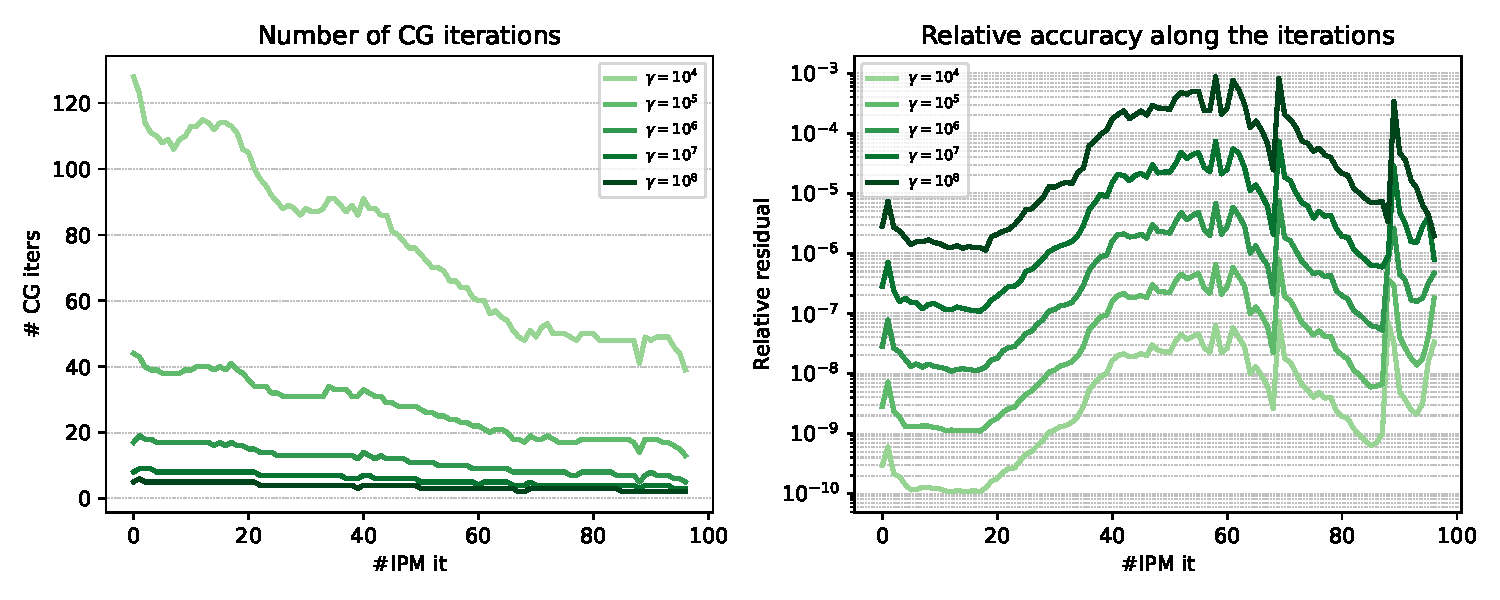
\includegraphics[width=\textwidth]{../figures/hybrid-gamma.pdf}
  \caption{
    Above: Decomposition of IPM solution time across
    (a) condensation time (cond.), (b) CG time, (c) total time
    spent in linear solver (linsol.) and (d) total time spent in
    IPM solver (IPM).
    Below: Impact of $\gamma$ on the total number of CG iterations
    and on the norm of the relative residual at each IPM iteration.
    The peak observe in the norm of the relative residual correspond
    to the primal-dual regularization performed inside the IPM algorithm,
    applied when the matrix $K_\gamma$ is not positive definite.
    \label{fig:hybrid:gamma}
  }
\end{figure}






\subsubsection{Equality relaxation strategy}
Assess the impact of $\varepsilon$ on the performance

\subsubsection{Performance profile}
Now, we look at a detailed performance profile that decomposes
the total running time spent at each iteration. Using the performance
profile, we highlight the bottlenecks of each KKT solvers.



\subsection{Benchmark on OPF instances}

\subsection{Benchmark on COPS instances}

\subsection{Discussion}

